
%! program = pdflatex

\documentclass[12pt]{article}
\usepackage{amsmath}
\usepackage{natbib}
\usepackage{graphicx}
\usepackage{amssymb}
\usepackage{epstopdf}
\usepackage{float} % to keep the figures in place

\usepackage{color}
\newcommand{\cred}{ \color{red}}
\newcommand{\cgreen}{\color{green}}
\newcommand{\cblue}{\color{blue}}
\newcommand{\cmag}{\color{magenta}}
\newcommand{\bn}{\begin{enumerate}}
\newcommand{\en}{\end{enumerate}}
\newcommand{\bi}{\begin{itemize}}
\newcommand{\ei}{\end{itemize}}
\newcommand{\be}{\begin{eqnarray}}
\newcommand{\ee}{\end{eqnarray}}
\newcommand{\by}{\begin{eqnarray*}}
\newcommand{\ey}{\end{eqnarray*}}
\renewcommand{\labelenumi}{(\alph{enumi}) }
%
\usepackage[margin=2.2cm, includehead]{geometry}% see geometry.pdf on how to lay out the page. There's lots.
\geometry{letterpaper} % or letter or a5paper or ... etc
% \geometry{landscape} % rotated page geometry
%\bibpunct{(}{)}{;}{a}{,}{,}
%\setlength{\textwidth}{16cm}
%\setlength{\textheight}{21cm}
\def\nonumber{\global\@eqnswfalse}
\newcounter{parnum}
\newcommand{\N}{%
  \noindent\refstepcounter{parnum}%
   \makebox[\parindent][l]{\textbf{[\arabic{parnum}]}}\quad  }
% Use a generous paragraph indent so numbers can be fit inside the
% indentation space.
\setlength{\parindent}{1.5em}

% See the ``Article customise'' template for come common customisations

\date{}
%\date{} % delete this line to display the current date

%%% BEGIN DOCUMENT
\usepackage{Sweave}
\begin{document}
\Sconcordance{concordance:check.tex:check.Rnw:%
1 47 1 1 0 25 1 1 8 1 2 4 1 2 2 4 1 2 2 4 1 2 2 14 1 1 2 1 0 2 1 1 2 8 %
0 1 1 7 0 1 2 4 1 1 2 1 0 1 1 4 0 1 2 1 1 1 2 7 0 1 2 2 1 1 2 5 0 1 2 3 %
1}

%\large
%\maketitle
\newtheorem{thm}{Theorem}[section]
\newtheorem{cor}[thm]{Corollary}
\newtheorem{lem}[thm]{Lemma}
\newtheorem{prop}[thm]{Proposition}
\newtheorem{defn}[thm]{Definition}
\newtheorem{exam}[thm]{Example}
\newtheorem{qstn}[thm]{Question}

%%%
\newpage
\begin{center}
{\bf Homework 3 - STAT 511}\\
Amal Agarwal
\end{center}
%==========================
\section*{Answer 1}
\bn
\item
Let us call y as the stopping distance (response variable) and x as the speed (predictor variable). For Exploratory Data Analysis (EDA) following scatter plots were obtained:
\begin{itemize}
\item Plot of y vs. x
\begin{figure}[H]
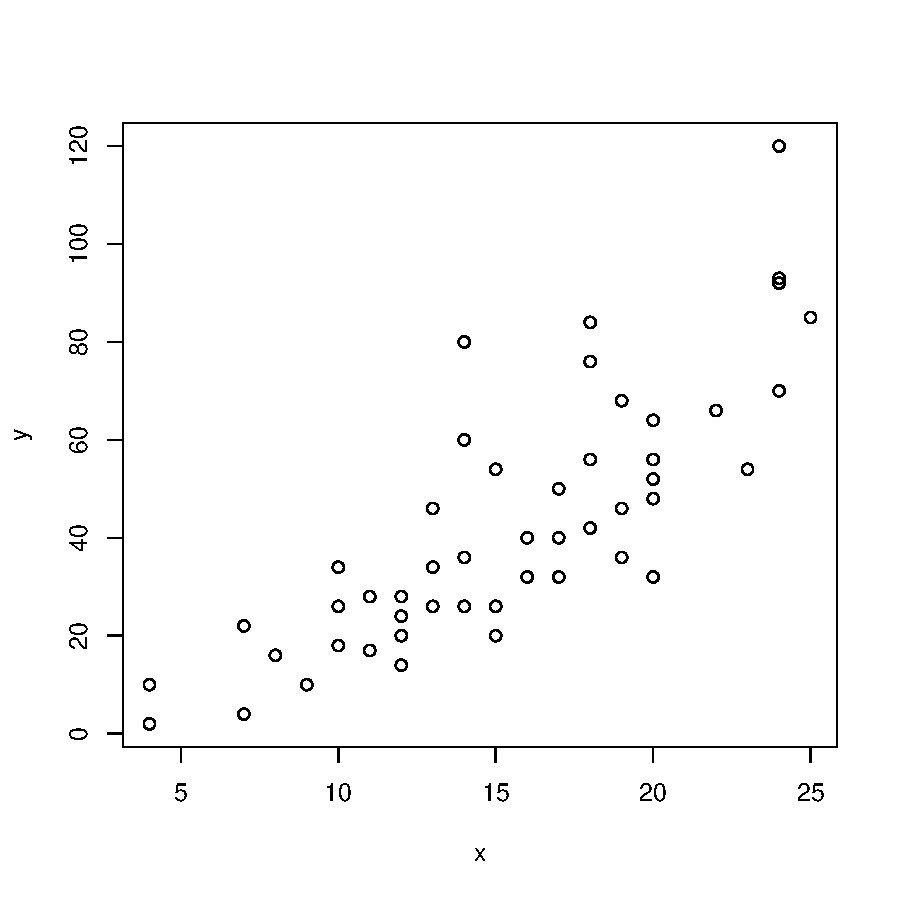
\includegraphics{check-001}
\end{figure}
\clearpage

\item Plot of $\sqrt{y}$ vs. x
\begin{figure}[H]
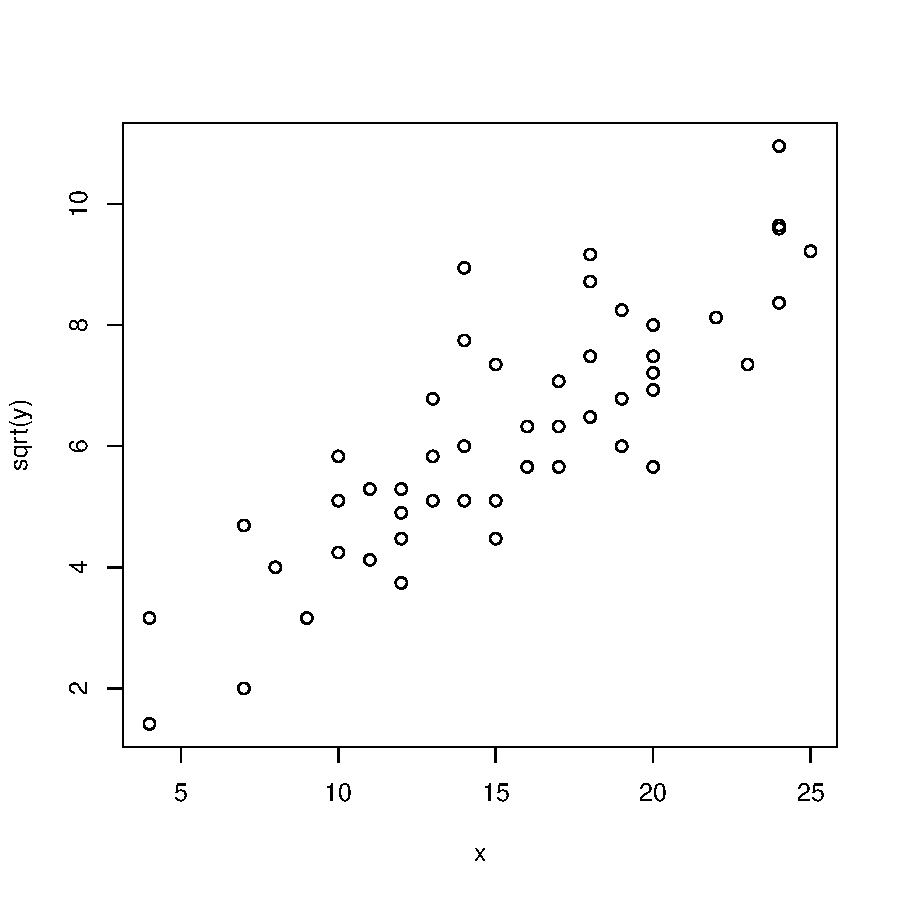
\includegraphics{check-002}
\end{figure}
\clearpage

\item Plot of $y$ vs. $x^2$
\begin{figure}[H]
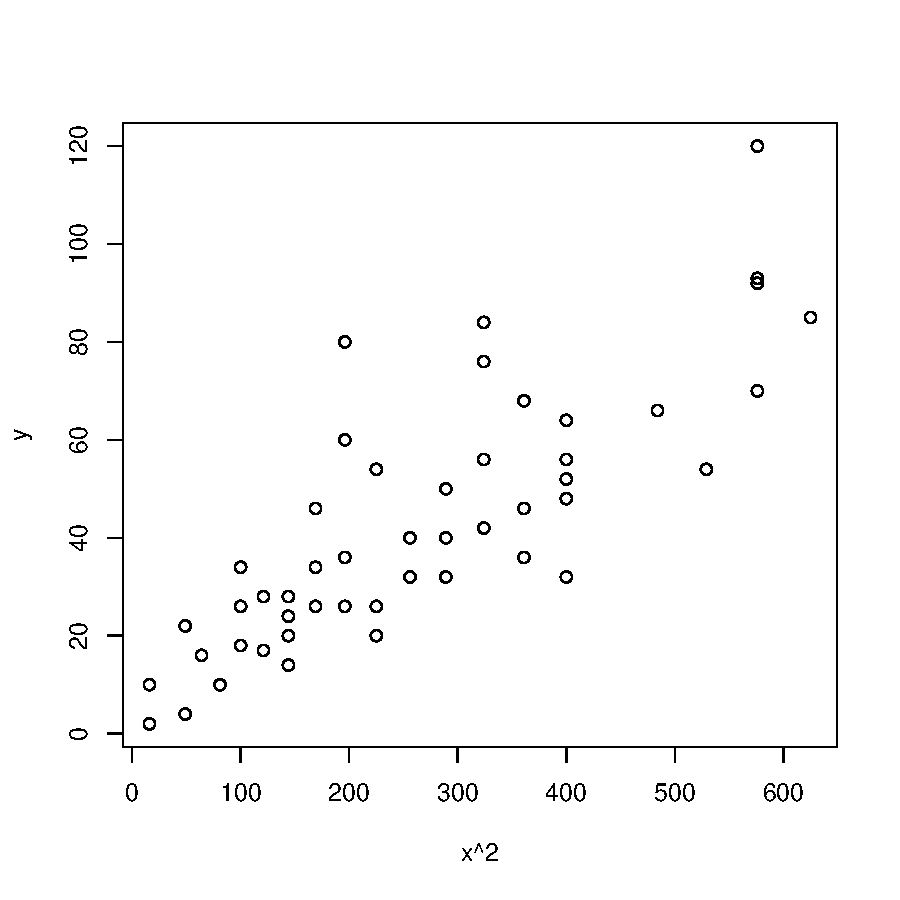
\includegraphics{check-003}
\end{figure}
\clearpage

\item Plot of $log(y)$ vs. x
\begin{figure}[H]
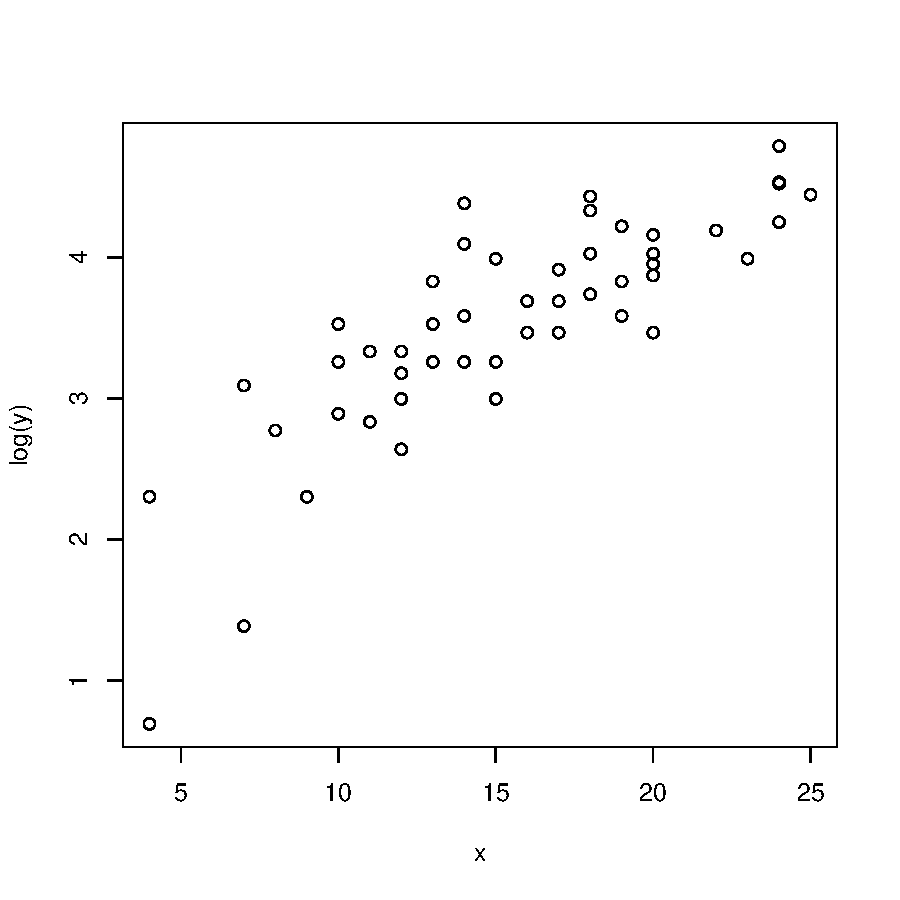
\includegraphics{check-004}
\end{figure}
\end{itemize}
It can be observed that the scatter plot of y vs. x does indicates a non linear relationship between y and x. Further tha density of data points for $x<7$ and $x>21$ is relatively lower than for $8<x<20$. The transformation $log(y)$ vs. x can be ruled out since it does not look linear. The transformation y vs. $x^2$ looks promising in terms of fitting a simple linear model. However, if I have to choose, the scatter plot that shows the most closest linear relationship after the transformation is $\sqrt{y}$ vs. x.

\item
The simple linear regression model in R that can be used to fit the given data is 
\begin{equation*}
\begin{aligned}
y &= \beta_0 + \beta_1 x + \epsilon
\end{aligned}
\end{equation*}

\clearpage
\item Using lm in R, to estimate model parameters and residuals.
\begin{figure}[H]
\begin{Schunk}
\begin{Sinput}
> fit1=lm(y~x)
> residuals=fit1$resid
> hist(residuals)
> ## the table given in summary(fit)
> summary(fit1)$coef
\end{Sinput}
\begin{Soutput}
              Estimate Std. Error   t value     Pr(>|t|)
(Intercept) -17.579095  6.7584402 -2.601058 1.231882e-02
x             3.932409  0.4155128  9.463990 1.489836e-12
\end{Soutput}
\begin{Sinput}
> summary(fit1)$sigma
\end{Sinput}
\begin{Soutput}
[1] 15.37959
\end{Soutput}
\end{Schunk}
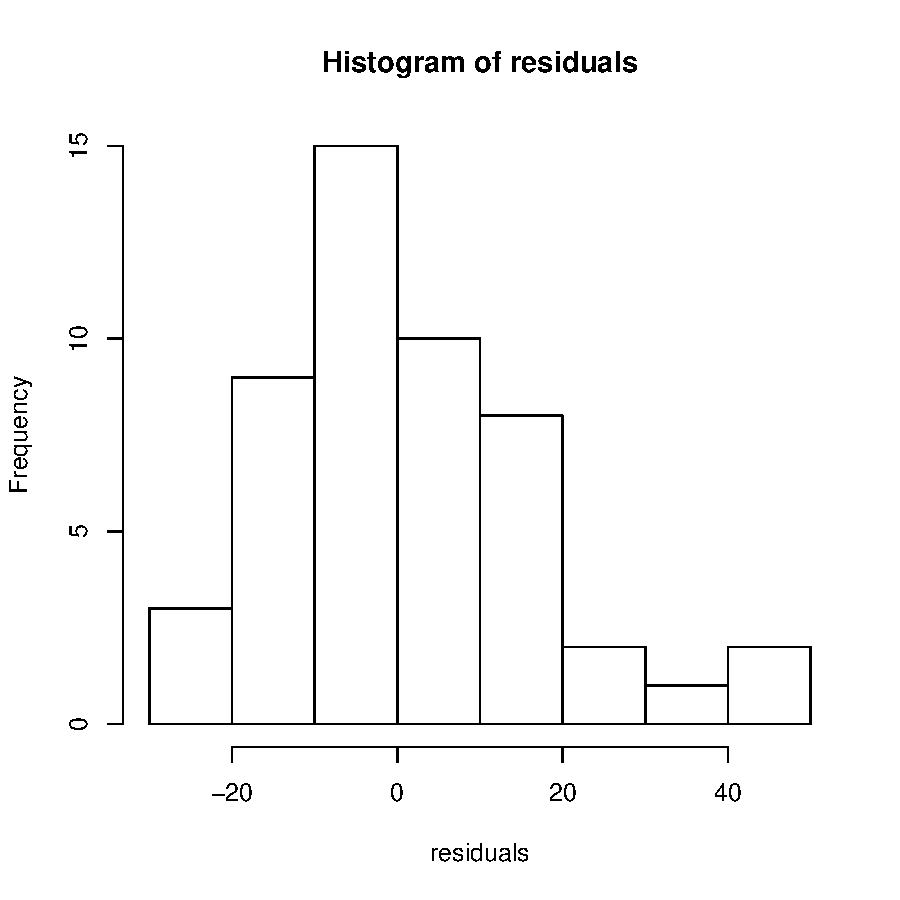
\includegraphics{check-005}
\end{figure}
\clearpage

\item
\begin{figure}[H]
\begin{Schunk}
\begin{Sinput}
> yhat=fit1$fitted.values
> plot(yhat,y)
\end{Sinput}
\end{Schunk}
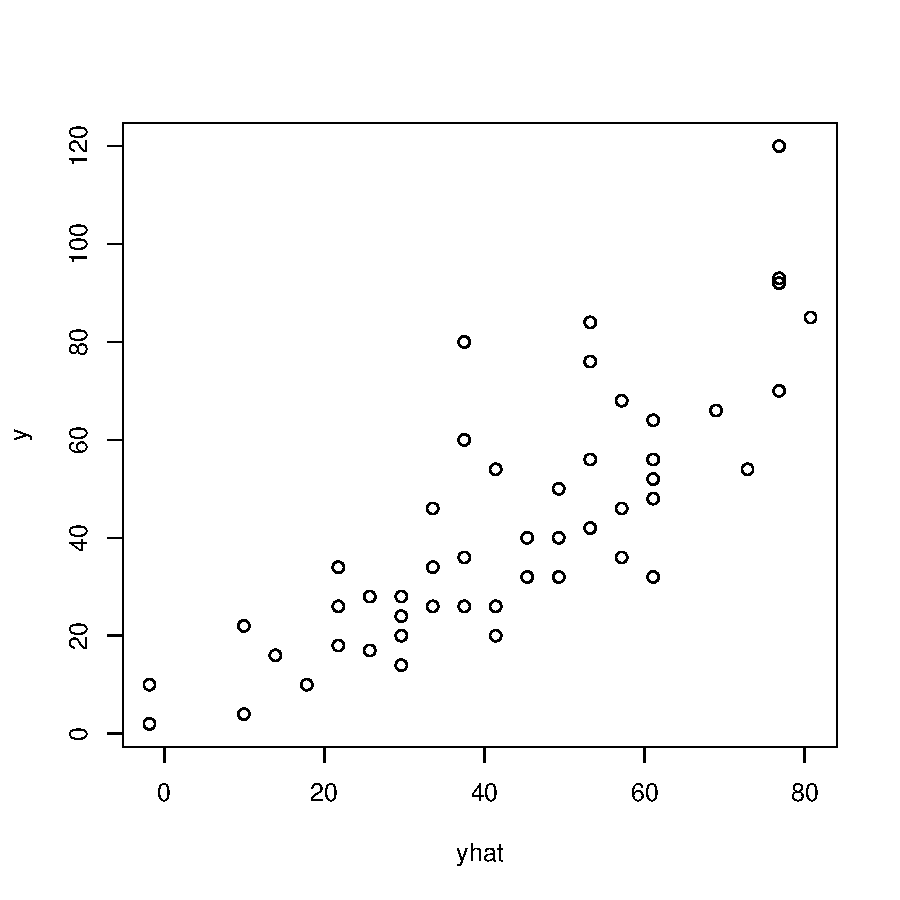
\includegraphics{check-006}
\end{figure}
The mean of residuals is given as
\begin{Schunk}
\begin{Sinput}
> mean(residuals)
\end{Sinput}
\begin{Soutput}
[1] 8.65974e-17
\end{Soutput}
\end{Schunk}
This is very close to zero which indicates that our assumption of $E(\epsilon)=0$ is satisfied.
To check for homoscedasticity, residuals can be plotted against x as
\begin{figure}[H]
\begin{Schunk}
\begin{Sinput}
> plot(x,residuals)
\end{Sinput}
\end{Schunk}
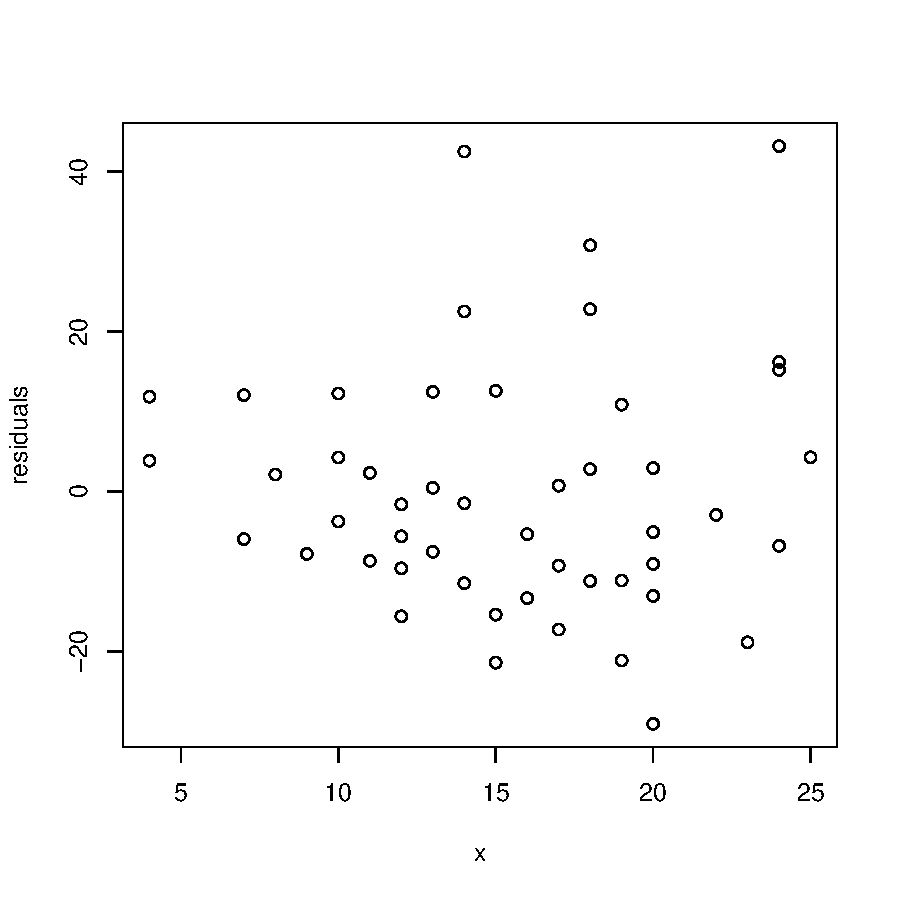
\includegraphics{check-008}
\end{figure}
Clearly, as x increases, the fluctuations of residuals around zero increases which implies that the estimated variance of the residuals increase with the covariate speed. This behaviour is called heteroscedascity which clearly violates our assumption of homoscedascity in the classical linear model.
\en
\end{document}
